\documentclass[a4paper, amsfonts, amssymb, amsmath, reprint, showkeys, nofootinbib, twoside]{revtex4-1}
\usepackage[english]{babel}
\usepackage[utf8]{inputenc}
\usepackage[colorinlistoftodos, color=green!40, prependcaption]{todonotes}
\usepackage[pdftex, pdftitle={Article}, pdfauthor={Author}]{hyperref}
\usepackage{amsthm}
\usepackage{mathtools}
\usepackage{physics}
\usepackage{xcolor}
\usepackage{caption}
\usepackage{hyperref}
\usepackage{multirow}
\usepackage{amsmath}
\usepackage{amssymb}
\usepackage{graphicx}
\graphicspath{Images}
\usepackage[left=23mm,right=13mm,top=35mm,columnsep=15pt]{geometry} 
\usepackage{adjustbox}
\usepackage{placeins}
\usepackage[T1]{fontenc}
\usepackage{float}
%\usepackage{longtable}
\usepackage{csquotes}
\usepackage{refstyle}
\usepackage{lipsum}

\begin{document}

\title{Study of Dielectric constant with frequency and Phase Transition  in $BaTiO_3$}
\author{Swaroop Ramakant Avarsekar}
\email{swaroop.avarsekar@niser.ac.in}
\affiliation{School of Physical Sciences, National Institute of Science Education and Research, HBNI, Jatni -752050, India}
\date{\today}
	
\begin{abstract}
In this experiment we study the frequency dependence of dielectric constant and ferro electric to para electric transition of $BaTiO_3$ and see the dielectric constant as function of temperature and frequency. We also determine Curie's Temperature for $BaTiO_3$ after which it undergoes phase transition from tetragonal to cubic lattice structure. The variation of capacitance with frequency for MLCC and Disc is also studied. The Curie's temperature was found to be $(135\pm3.85\%)^\circ C$.
\end{abstract}
	
\keywords{Perovskite, Curie tempertaure, Permitivity, Schering Bridge}
	
\maketitle

\section{Theory}
Permittivity of a material is the tendency of its charge to distort in presence of an electric field. Dielectric constant $\epsilon$ of a material is the ratio of permittivity of the material to the permittivity of free space. A high dielectric constant suggests that the material has a high ability to screen charges. Lower dielectric constant is preferred for use in capacitors and other electric appliances as the electric loss is lower. However, in case for lower values of capacitors, high dielectric constant is also used. Permittivity is a complex property with imaginary part signifying energy loss and real part signifying energy stored. The real part is dependent on the polarizability of the material.
The polarizabilty can be classified into
\begin{enumerate}
\item Electronic polarization occurs when an electric field displaces the nucleus w.r.t the electrons of its atom.
\item Atomic polarization occurs when the positive and negative charges are attracted in opposite directions due to an electric field.
\item  Permanent Dipole occurs due to the unbalanced sharing of electrons in the atom.
\item Space charge polarization occurs when the material is made of more than one component and the charge carriers become trapped between their interface.
\end{enumerate}
Each has its own characteristic relaxation frequency. As frequency increases, some of these drop off. The dielectric permittivity at optical frequencies arises almost entirely from the electronic polarizability or space charge polarization.
The imaginary part of permittivity is also used in applications such as microwave heating etc. The ratio of the imaginary part to the real part suggest the ability of the material to convert electromagnetic radiation to heat. Dissipation factor is defined as
\begin{equation}
	tan\delta=\frac{Im(\epsilon)}{Re(\epsilon)}
\end{equation}

\begin{figure}[H]
	\centering
	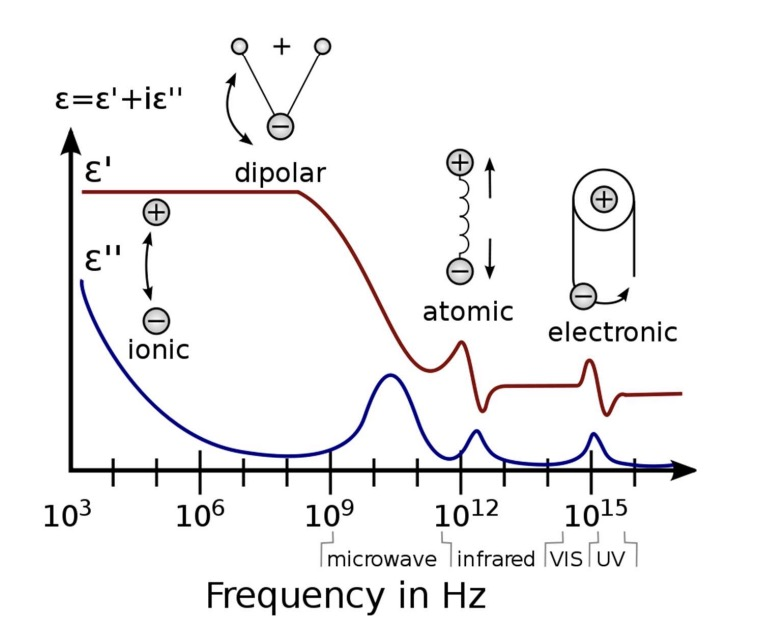
\includegraphics[scale=0.34]{1}
	\caption{Real and imaginary part of permittivity as function of frequency. }
	\label{1}
\end{figure}

Barium Titanate (BT), has perovskite structure with large dielectric constant. Perovskite is originally calcium titanate of the form $ABO_3$, where A site occupy corners of cube, B site cation occupy body centre. BT has ferroelectric tetragonal phase below its curie point and paraelectric cubic phase. As the BT ceramics have a very large room temperature dielectric constant, they are mainly
used in multilayer capacitor applications. The grain size control of these polycrystalline sample
used in the experiment is very important for these applications.  

\begin{figure}[H]
	\centering
	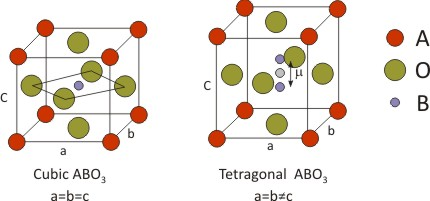
\includegraphics[scale=2.2]{2}
	\caption{Perovskite structure $ABO_3$ }
	\label{1}
\end{figure}

\begin{figure}[H]
	\centering
	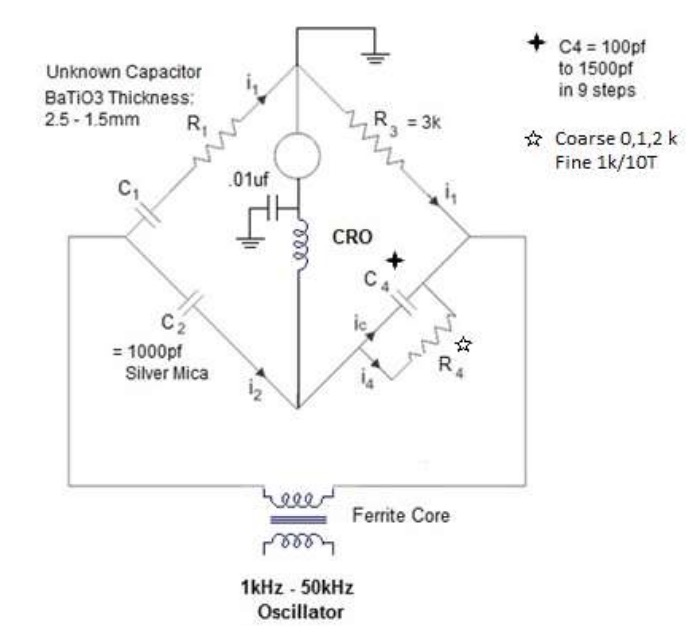
\includegraphics[scale=0.35]{3}
	\caption{Schering Bridge}
	\label{1}
\end{figure}

The Schering bridge is an electrical circuit which can be used to determine the capacitance of an unknown capacitor, by balancing the current passing through the arms of the circuit. By balancing the four arms of the circuit, with appropriate value of capacitance and resistance, we have,
\begin{align}
	\frac {C_1}{ C_2}=\frac{R_3}{R_4}\\
	\frac {R_1}{ C_3}=\frac{C_4}{C_2}
\end{align}

where $C_1$ is unknown capacitance, $C_2$ is standard silver mica capacitor of 1000 pF, $C_4$ is variable capacitor, $R_3$ is metal film resistor of 3k$\Omega$ and $R_4$ is variable resistance. 

The dissipation factor is calculated from,
\begin{equation}
	\text{Dissipation factor}=\omega C_1R_1=\omega C_4R_4=2\pi f (CR)
\end{equation}
\\
Diffuseness factor is slope of $ln(T-T_C)$ versus $ln(\frac{1}{\epsilon}-\frac{1}{\epsilon_m})$, where $T_C$ is curie temperature and $\epsilon_m$ is maximum dielectric constant. 

\section{Experiment and Analysis}

Refer attached table for observations.

\begin{figure}[H]
	\centering
	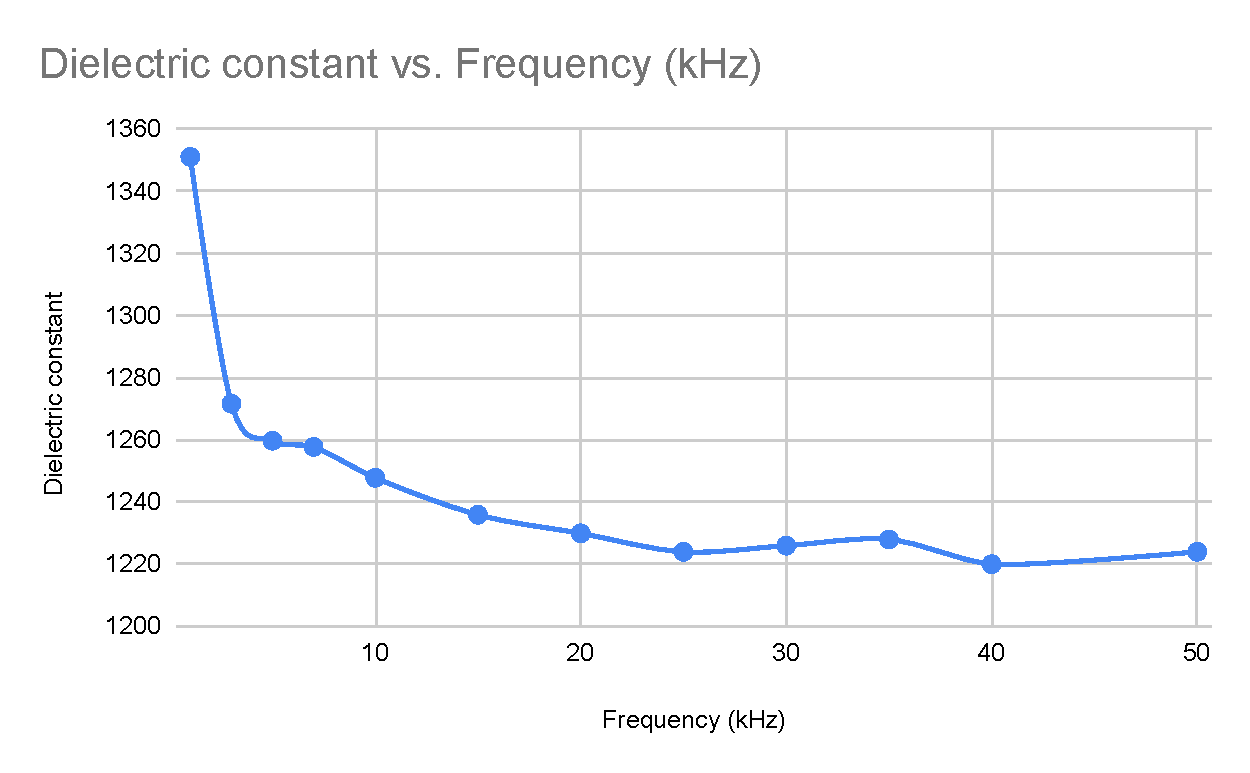
\includegraphics[scale=0.4]{a}
	\caption{Variation of dielectric constant with frequency for BT}
	\label{1}
\end{figure}

\begin{figure}[H]
	\centering
	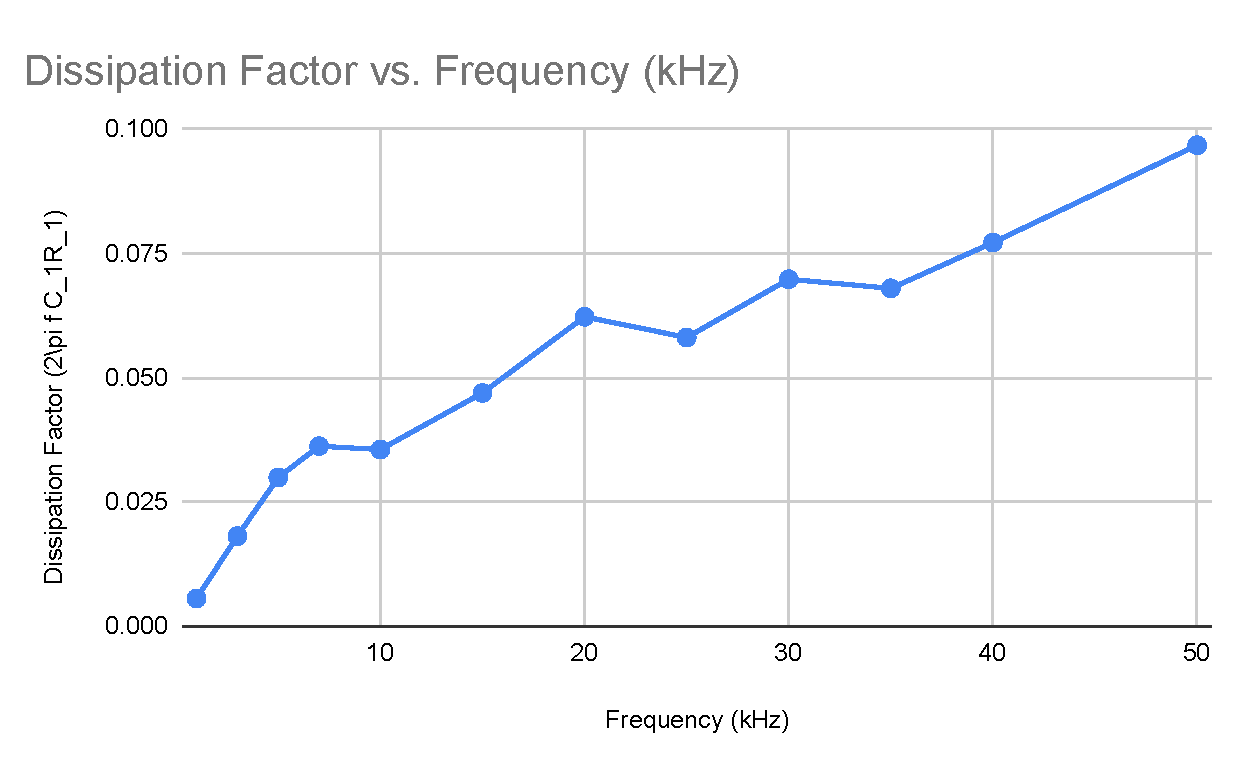
\includegraphics[scale=0.4]{f}
	\caption{Variation of dissipation factor with frequency for BT.}
	\label{1}
\end{figure}

\begin{figure}[H]
	\centering
	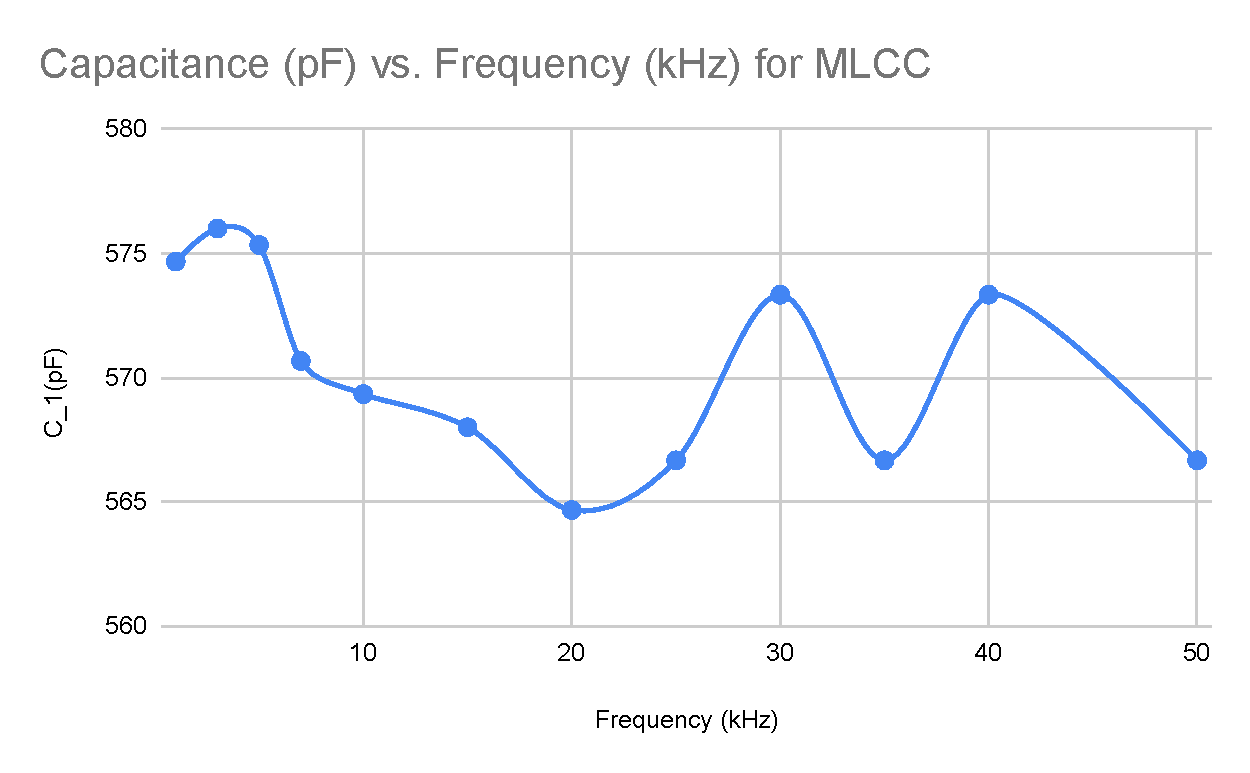
\includegraphics[scale=0.4]{m}
	\caption{Variation of Capacitance with frequency for MLCC}
	\label{1}
\end{figure}

\begin{figure}[H]
	\centering
	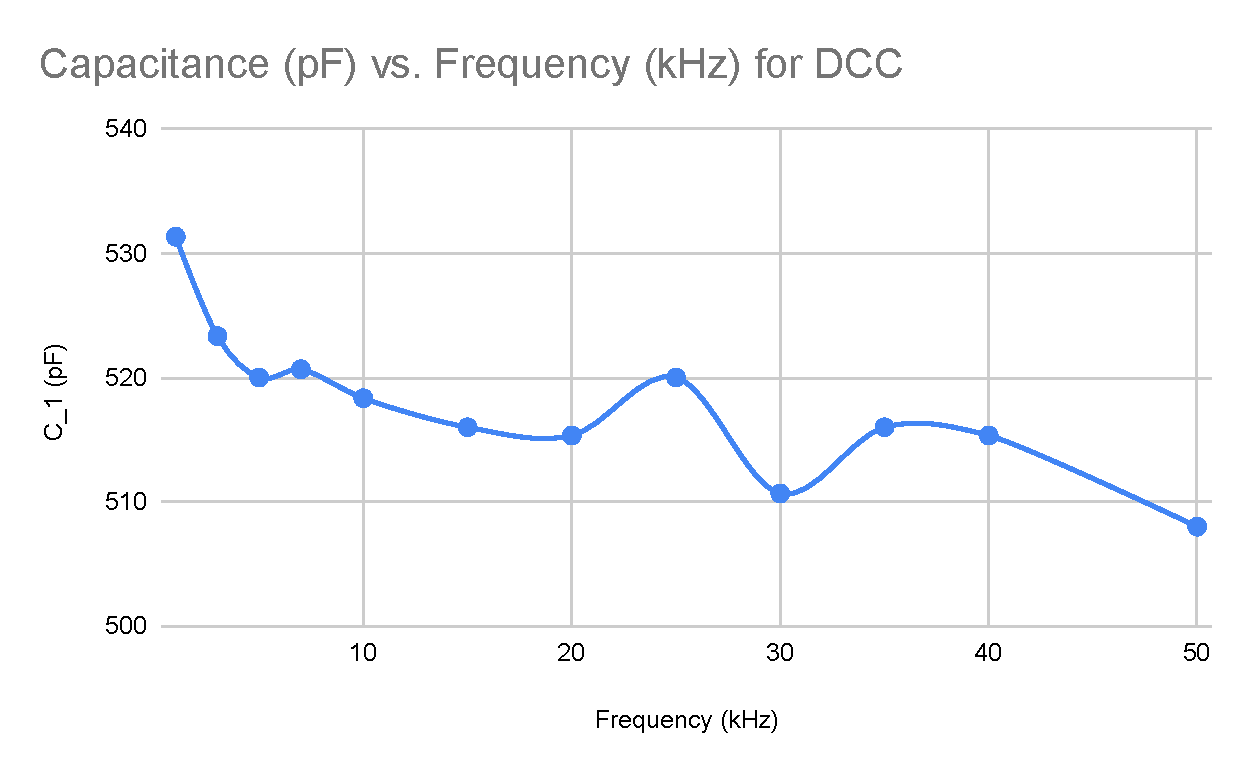
\includegraphics[scale=0.4]{d}
	\caption{Variation of Capacitance with frequency for Disc.}
	\label{1}
\end{figure}

\begin{figure}[H]
	\centering
	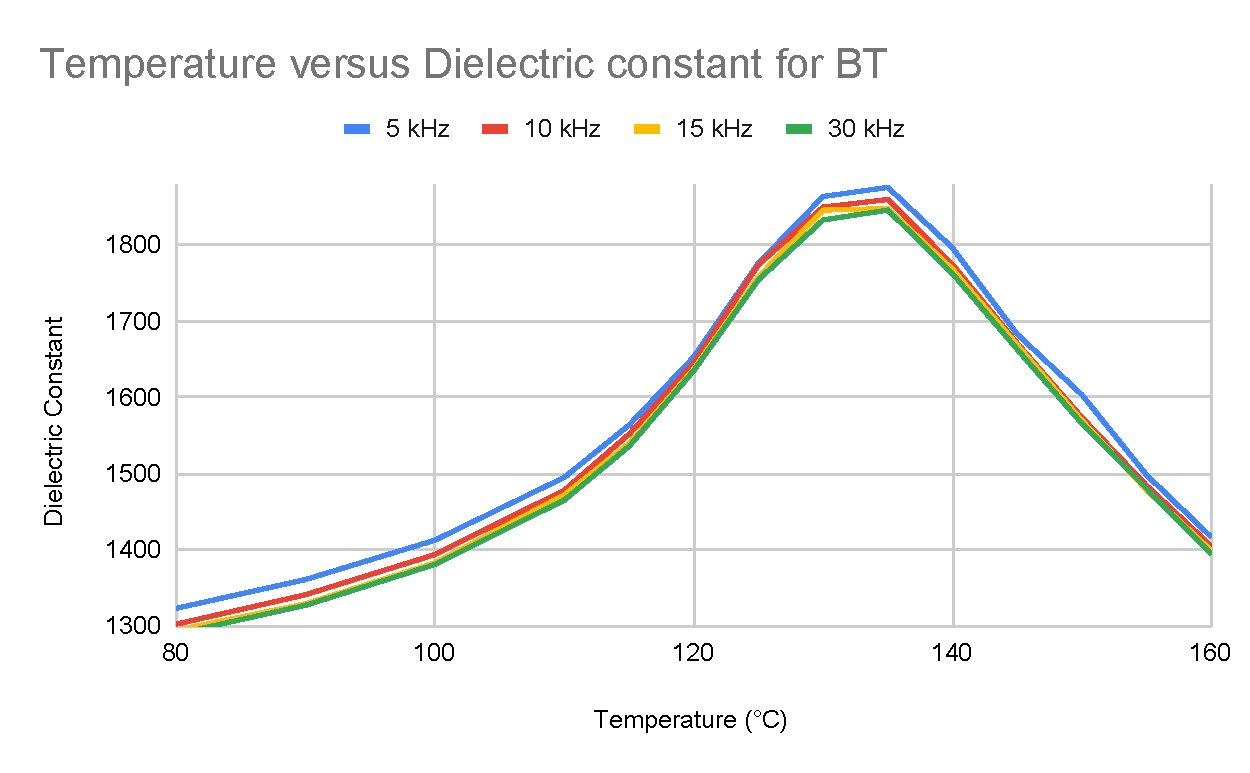
\includegraphics[scale=0.42]{c}
	\caption{Plot of Dielectric constant as a function of Temperature for different frequencies}
	\label{1}
\end{figure}

\begin{figure}[H]
	\centering
	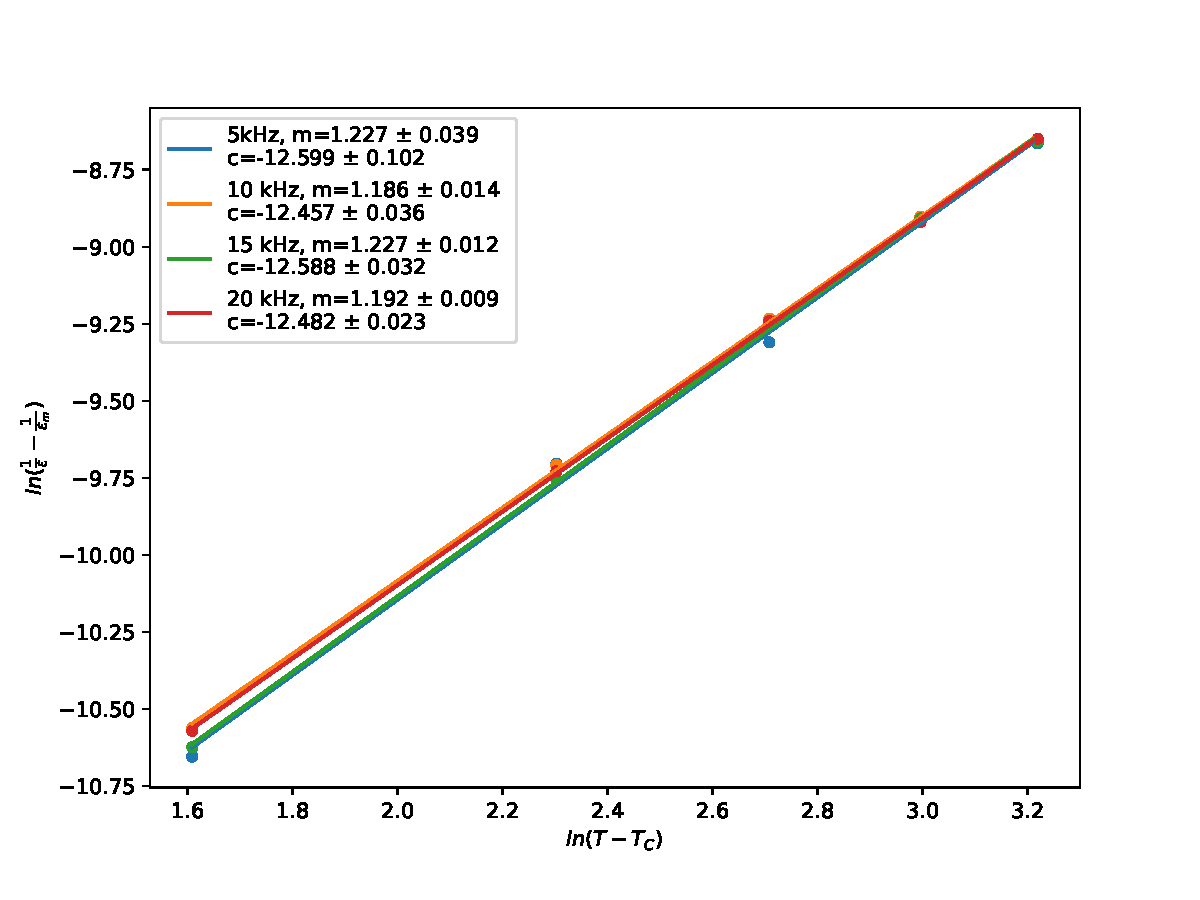
\includegraphics[scale=0.5]{ln}
	\caption{Plot of diffuseness parameter}
	\label{1}
\end{figure}

Figure (4) shows the variation of dielectric constant with frequency for BT. It is seen that as frequency is increased from range 1-50 kHz. Dielectric constant decreases with in increase in frequency. The same is expected for plot of capacitance versus frequency for MLCC and Disc as shown in figure (6) and figure (7). This behavior is caused due to space charge polarization caused by mobile charge carriers whose motion is impeded by interface due to grain or phase boundary. Figure (5) shows that dissipation factor of BT increases with frequency reflects increses in friction between dipoles due to their inability to follow up the first variation of the applied alternating electric field.

We also studied the temperature dependence of dielectric constant of BT. It was seen that the dielectric constant was maximum at T= 135 $^\circ C$ irrespective of frequency. Here, temperature dependence of four frequencies were considered. The dielectric constant increases with temperature attains maximum at Curie's temperature where it undergoes tetragonal to cubic structure, and decrease the dielectric constant. The literature value of Curie's temperature for BT is 130$^\circ C$.
Therefore relative error (RE) is calculated as -
\begin{equation}
	RE=\frac{135-130}{130}100\%=3.84\%.
\end{equation}

The relative error could be reduced by taking smaller temperatures approaching close to the literature value.

Diffuseness factor is slope of $ln(T-T_C)$ versus $ln(\frac{1}{\epsilon}-\frac{1}{\epsilon_m})$, where $T_C$ is curie temperature and $\epsilon_m$ is maximum dielectric constant. The plot is valid for temperatures above Curie's temperature only. The slope for different frequencies are as follows-

\begin{align}
\text{For 5 kHz}=1.227\pm0.039\\
\text{ For10 kHz}=1.186\pm0.014\\
\text{For 15 kHz}=1.227\pm0.012\\
\text{For 20 kHz}=1.192\pm0.009\\
\end{align}

\section{Conclusion}
We studied the frequency dependence of dielectric constant and ferroelectric to para-electric transition of $BaTiO_3$ and see the dielectric constant as function of temperature and frequency. It was seen that with increase in frequency, the dielectric constant decreased and dissipation factor increases. The variation of capacitance with frequency for MLCC and Disc also decreases with frequency except few bumps due to doping with different dielectrics and impurities. We also determine Curie's Temperature for $BaTiO_3$ after which it undergoes phase transition from tetragonal to cubic lattice structure. The Curie's temperature was found to be ($135\pm3.84\%)^\circ C$, which is constant irrespective of frequencies. Finally we plot $ln(T-T_C)$ versus $ln(\frac{1}{\epsilon}-\frac{1}{\epsilon_m})$ to get the diffuseness factor, which is a linear plot. For 5 kHz, we got slope as $1.227\pm0.039$, for 10 kHz=$1.186\pm0.014$, for 15 kHz $1.227\pm0.012$ for 20 kHz, $1.192\pm0.009$. The error in diffuseness factor is minimal.

Some sources of error in this experiment could be improper contact with the sample, fluctuations in temperature, loose connections and poor Schering bridge apparatus. Make sure to ensure stable input. Few precautions have to be considered, such as the spring probe should be place gently on the sample. The resistance should not be increased more than 2 k$\Omega$.

\section{References}
\begin{enumerate}
\item{SPS NISER Lab Manual}
\item\url{https://archive.nptel.ac.in/content/storage2/courses/113104005/lecture25/images/figure6.jpg} \item {\url{https://en.wikipedia.org/wiki/Perovskite}}

\end{enumerate}

\end{document}